\section{Calculating the attributes}\label{sec:calculations}

Before the program can evaluate the routes, it needs to calculate the attributes of the different routes as mentioned in
the flowchart in Figure~\ref{fig:evaluate}.
This is a relatively difficult task, as the program needs to calculate the distance, price and \unit{CO_{2}} emission.
Some attributes are easier to calculate than others, but they all require some form of calculation.

Rejseplanen has systems in place to calculate some of those attributes, but the API does not provide them.
This means that we have to calculate them ourselves by our own means.
Our calculations will not be 100\% accurate, as we have simplified some calculations, but they will be close
enough for our purposes.

\subsection{Calculating distance}\label{subsec:calculating-distance}

The program needs the distance of a route for the calculations.
As we don't use a map API, the program can't properly calculate the distance between two points.
This means that the program has to ignore roads and instead calculate the distance by the train tracks.
The problem is that Rejseplanen only provides the coordinates of the stations, not the tracks, why we decided to instead
calculate the distance between these coordinates.
The disadvantage of the approach is, that it won't account for curves along the track, as the distance is calculated as
a straight line between the stations.
An example of how the distance is going to look can be seen in Figure~\ref{fig:image-google-maps-distance-calculation}.

\begin{figure}[H]
    \centering
    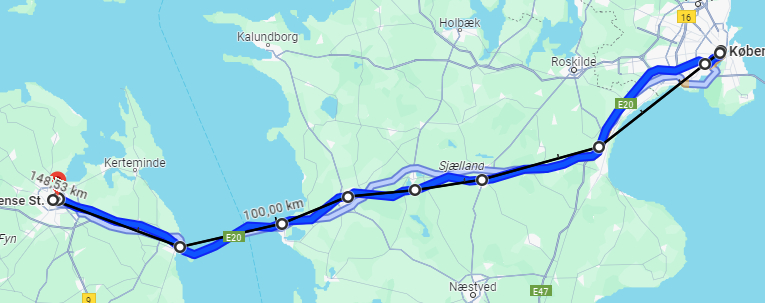
\includegraphics[width=0.8\textwidth]{images/google-maps-distance-calculation}
    \caption{A route between Copenhagen and Odense. \\ Blue line is Google Maps' distance, black line is our distance.}
    % TODO fix the text not being centered
    \label{fig:image-google-maps-distance-calculation}
\end{figure}

The way we decided to calculate what the distance, is by using the Haversine formula~\cite{haversine}.
The formula is used to calculate the distance between two points on a sphere.
We'll be using the coordinates from Rejseplanen to calculate the distance between two stations.
The formula is as follows:

\begin{equation}
    haversine(\theta) = sin^{2}(\frac{\theta}{2})
\end{equation}

The program will use it to calculate the distance between two points using the following formula:

\begin{equation}
    (\frac{d}{r}) = haversine(\phi_{2} - \phi_{1}) + cos(\phi_{1}) \times cos(\phi_{2}) \times haversine(\lambda_{2} - \lambda_{1})
\end{equation}

Where \(\phi\) is the latitude, \(\lambda\) is the longitude, \(d\) is the distance and \(r\) is the radius of the
Earth, which is about 6371 km.

\subsection{Calculating price}\label{subsec:calculating-price}

Calculating the price is a lot more difficult than calculating the distance.
As Denmark's public transport network is divided into zones, the price is calculated based on how many zones you travel
through on a given journey.
The price is also affected based on a number of different variables, such as age, region, occupation and more.
For our program, we decided to calculate the prices for Pendlerkort and Ungdomskort.

\subsubsection{Zones}

To calculate the price then is to figure out how many zones a journey passes through.
Unfortunately, Rejseplanen's API does not provide any information about how many zones a route goes through, why the
decision was made to calculate the average size for a zone.
As the zones are not all the same size, the number of zones a route passes through may be slightly off.
However, this is the best option to circumvent adding further complexity to our program.

Our somewhat primitive solution to achieve an average zone size, is calculated by picking two stations at random and
counting how many zones the route goes through using DSB's zone map~\cite{price_zones}.
We then used Google Maps to provide us the distance along the tracks between two stations.
Finally, we divided the distance by the number of zones to get the average size of a zone along the route.

\begin{figure}[H]
    \centering
    \noindent
    \begin{tabular}{ || c | c | c || }
        \hline
        Route & Zones and distance & Zone size \\
        \hline\hline
        Korsør to Ringsted & 5 zones 45 km & 9 km per zone \\
        \hline
        Ringsted to Køge Nord & 6 zones 30 km & 5 km per zone \\
        \hline
        Kalundborg to Holbæk & 7 zones 45 km & 6.4 km per zone \\
        \hline
        Frederikssund to Kbh & 10 zones 23 km & 2.3 km per zone \\
        \hline
        Voldingborg to Ringsted & 8 zones 52 km & 6.5 km per zone \\
        \hline\hline
        Zone Averages & & 6 km per zone \\
        \hline
    \end{tabular}
    \caption{Table of our calculations of zone size averages.}
    \label{fig:table-zone-size-averages}
\end{figure}

From Figure~\ref{fig:table-zone-size-averages} we determined that the average size of a zone is roughly about 6
kilometers.
As mentioned, this way of calculating the price of a trip is not ideal, as the sizes of zones varies a lot.
This will provide some price differences compared to the real price of trips, primarily in the city of Copenhagen,
as the zones there are considerable smaller than outside, and as more people live there.

\subsubsection{Pendlerkort price}

Another aspect of the price calculation is the price for Pendlerkort.
This card allows commuters to freely travel between a set amount of zones, be that with bus or train.
Rejseplanen has a website where the user can input their route, and it'll calculate the price for the
Pendlerkort~\cite{price_calculator}.
As the prices provided by Rejseplanen and DSB in the tables in Figure~\ref{fig:table-rejseplanen-price-calculations} and
Figure~\ref{fig:image-dsb-pendlerkort-pris} are accurate enough, they are hard-coded into the program.

\begin{figure}[H]
    \centering
    \noindent
    \begin{tabular}{ || c | c || }
        \hline
        Route & Zones and price \\
        \hline\hline
        Odense to København & 30 zones 3750 DKK \\
        \hline
        Køge Nord to København & 9 zones 1470 DKK \\
        \hline
        Græsted to Vordingborg & 18 zones 3000 DKK \\
        \hline
        Aarhus to København & 51 zones 4590 DKK \\
        \hline
    \end{tabular}
    \caption{Table of Rejseplanen's price calculations.}
    \label{fig:table-rejseplanen-price-calculations}
\end{figure}

\begin{figure}[H]
    \centering
    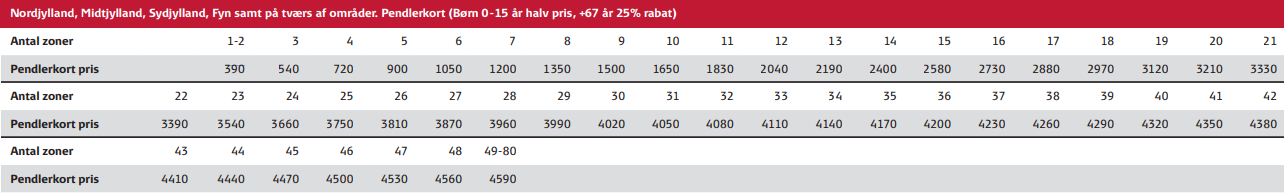
\includegraphics[width=1\textwidth]{images/dsb-pendlerkort-pris.jpg}
    \caption{Price of Pendlerkort per zones~\cite{price_sheet}.}
    \label{fig:image-dsb-pendlerkort-pris}
\end{figure}

\subsubsection{Ungdomskort price}

Ungdomskort is a type op Pendlerkort that is primarily aimed at young people or students.
The price is significantly lower than Pendlerkort, so we deemed it necessary to implement it in our program.
The program prompts the user if they're a student, and if they are, this will be included in the price calculations.
Calculating the price for Ungdomskort is a lot easier than Pendlerkort, as the method is listed on their
website~\cite{price_ung}.

The price is calculated by taking the equivalent price for a Pendlerkort and then taking 2487 DKK from it.
Then the result is halved, and finally 663 DKK is added to the result.
Here's an example for a Pendlerkort between Odense and Copenhagen, that costs 3750 DKK:

\begin{equation}
    \frac{3750 - 2487}{2} + 663 = 1294 \text{DKK}
\end{equation}

\subsubsection{Car and bike price}

As commuting also entails individuals who do not use public transport, the program also need to calculate the price for
cars and bikes.
Included in the calculations for the price of a car is price of gas or electricity, insurance and maintenance.
As the pricing can vary a lot depending on different circumstances, so we'll use an average price.

According to Global Petrol Prices, the average price for gas in Denmark is 12.20 DKK per liter~\cite{price_gas}, however
looking at the graph, it seems that recently the prices have been around 14 DKK, so we'll choose that number for our
calculations.
This is once again not an ideal way to calculate the price, but to limit further complexity this is our best option

The calculation uses the cars fuel efficiency as inputted by the user as seen in Figure~\ref{fig:input}.
Our program will calculate the price of a car by dividing the distance by the fuel efficiency, and then multiply it by
the price of gas.
The calculation will time by two to account for both way travel.
Finally, the program multiplies the price by 20, to account for the duration of work month.
Below is an example of a commute that is 30 km long with a fuel efficiency of 17 km per liter and a gas price of 14 DKK.

\begin{equation}
    \frac{30}{17} \times 14 \times 40 = 988 \text{DKK}.\label{eq:equation}
\end{equation}

While electric cars don't require gas, they do require electricity.
The most popular electric car in Denmark, the Tesla Model 3, which has an efficiency of 142 miles per gallon equivalent
(MPG-e), which is about 60 km per liter equivalent~\cite{price_el}.
One gallon is the equivalent of 33.7 kWh~\cite{price_mpge}, which is 8.9 kWh per liter.
With that in mind, we can use the price of electricity in Denmark, which is 2.8 DKK per kWh~\cite{price_energy}, to
calculate that the cost per km for electric cars is 24.9 DKK.

Another big factor for the insurance price depends on the type of subscription the user has.
The average cost is roughly 250 DKK per month~\cite{price_insurance}.
When it comes to maintenance, the average cost is about \$1064~\cite{price_repair}, which equals to 600 DKK per month.
This amounts to 850 DKK that the user has to pay on top of the gas or electricity prices for the month.

Bikes in comparison are a lot cheaper, as they don't require insurance or gas.
However, they do require maintenance.
Compared to cars, maintenance for bikes is a lot cheaper.
According to The Pro's Closet, they've estimated that the average cost of maintenance for a road bike is about \$185 per
year~\cite{price_bike}.
This converts to about 1200 DKK per year, which is 100 DKK per month.

\subsection{Calculating time}\label{subsec:calculating-time}

Calculating the time is marginally easier than calculating the distance, but only for trains.
Rejseplanen provides a time for when the train arrives at the station, and when it departs.
Trivially, the difference in these time stamps is then the time it takes.
However, for cars and bikes, we need to calculate the time ourselves.
This is done by dividing the distance by the average speed of a car or bike.
For the sake of minimizing complexity in the calculations, it is assumed that the user will be using the highway, when
commuting by car.

It is also assumed that the user will spend around 15 minutes to get out of the city, and 15 minutes to get into the
next city.
Therefore, for the first 30 minutes, the calculations will apply the average speed of a car in the city, and
afterward apply the average speed of a car on the highway.
The average speed of a car on the highway is about 120 km/h~\cite{time_highway}, and the average speed of a car in
the city is about 35 km/h~\cite{time_city}.

Depending on the distance, bike and walking time estimations is rather complicated.
This is already the case with for example Google Maps, where the time it takes to walk a distance does not include
breaks or sleep when addressing large distances by foot or by bike, resulting in a vastly smaller time estimate.
A 100 km trip is estimated to take 23 hours by foot, but it'll realistically take longer, when accounting for breaks
and exhaustion.

Walk and bike speed can vary by age and sex.
It is therefore assumed that the average walking speed is 4.6 km/h, which is accurate for people up to 50 years of age
~\cite{time_walk}.
As for biking, the speed can vary by the bike and the biker's experience too.
It is therefore assumed that the average speed for a normal bike tour is 17.5 km/h~\cite{time_bike}.

\subsection{Calculating CO2 emission}\label{subsec:calculating-co2-emission}

The final attribute we need to calculate is the \unit{CO_{2}} emission.
Public companies, such as DSB, have to report their \unit{CO_{2}} emission, why the programs calculations will be based
on these audited reports.
The list below is a sample of the different types of public transport vehicles and their \unit{CO_{2}} emissions per
person per kilometer as seen in Table~\ref{tab:emissions}.

\begin{table}[H]
    \centering
    \begin{tabular}{ || c | c || }
        \hline
        Vehicle type & \unit{CO_{2}} pr. person pr. km \\
        \hline\hline
        S-train & 14 gram~\cite{dsb2023} \\
        \hline
        Regional train & 38 gram~\cite{dsb2023} \\
        \hline
        InterCity train & 29 gram~\cite{dsb2023} \\
        \hline
        Speed train & 37 gram~\cite{dsb2023} \\
        \hline
        Long distance bus & 23 gram~\cite{cowi2022} \\
        \hline
        City bus & 10 gram~\cite{ntm2023} \\
        \hline
    \end{tabular}
    \caption{\unit{CO_{2}} pr. person pr. km. pr. vehicle type.}
    \label{tab:emissions}
\end{table}

Since the data is per kilometer, we can multiply the distance by the \unit{CO_{2}} emission to get the total
\unit{CO_{2}}.
Afterward 40 (20 work days in a moth times 2 way travel) is multiply to this total, similar to the price calculation, to get the
\unit{CO_{2}} emission for a month.
This total is finally converted to kilograms to increase readability.

When it comes to car emissions, the fuel efficiency is used to calculate the \unit{CO_{2}} emission.
For a diesel car, one liter of diesel creates 2.68 kg of \unit{CO_{2}}~\cite{co2_car} when used as car fuel.
Similarly to the other calculations, the total is multiplied by 40 (20 work days in a moth times 2 way travel) to get
the \unit{CO_{2}} emission for a whole month.

As for electric cars, they don't emit any \unit{CO_{2}}, why this emission value is set to 0 by default.
